\chapter{Neutronics Feature Selection} \label{ch:sweeps}
A valid reactor design must meet certain neutronics constraints. The main
neutronics constraint is reactivity. The reactor must be able to sustain a chain
reaction from startup, to the final second of the 10 year lifetime. End of Life
(EOL) reactivity was the target metric for the neutronic design of the core.
Traditional reactor design processes will spend a long time tweaking neutronics
parameters to meet certain system requirements. The total mass optimization
needed a rapidly excecutable model that could respond to various inputs.
This meant it was important to understand how a reactor's neutronic
performance is impacted by various input and design parameters in order to
construct a reduced-order neutronics model that could be used in the mass
optimization routine. A 5-dimensional 
sampling was conducted in order to select important predictors for EOL
reactivity.

\section{Parametric Study of Neutronics Parameters}
Homogeneous MCNP6.1 depletion models were used to analyze the EOL \keff response
to neutronics parameters (predictors). The core region was homogenized and
surrounded by a graphite reflector. A large set of 5-dimensional predictors and
EOL \keff results was produced to investigate the neutronics parameter space.
These predictors and their results helped develop an understanding of the
reactor response to important design and operational parameters. High Throughput
Computing capabilities at UW were used to perform 3901 depletion calculations
with MCNP6.1. Each model represented a unique sampling in every dimension using
the Latin Hypercube Sampling (LHS) technique\citep{LHS}. The LHS technique ensured even
sampling for every dimension. The sampled and fixed dimensions/parameters are
shown in Table \ref{tab:lhs_sweep_vars}.

\begin{table}[h]
  \centering
  \caption{Homogeneous Geometry and Depletion Parameters}
  \begin{tabular}{ll}
    \toprule
     Core Radius                		   & 10 - 50 [cm] \\
     Fuel Enrichment 					   & 20\% - 90\% $^{235}$U\\
     Coolant Channel Radius                & 0.5 - 1 [cm] \\
     Fuel Pitch to Coolant Channel D.      & 1.1-1.6 [-]\\
     Thermal Power						   & 80-200 [kW]\\
     Reflector Thickness				   & 15 [cm]\\
     Core Aspect Ratio					   & 1 [-] \\
     Fuel Temperature					   & 300 [K]\\
     Reactor Physics Code, Data			   & MCNP6.1, ENDF-7.2
  \end{tabular}
  \label{tab:lhs_sweep_vars}
\end{table}

\section{Parametric Study Results}
The target metric for the neutronics sampling was EOL \keff $\geq$ 1.0. In
order to determine the dependence of EOL \keff on each swept parameter in Table
\ref{tab:lhs_sweep_vars}, EOL \keff was plotted against the parameters.

\subsection{Uranium 235 Mass}
The strongest predictor of EOL \keff is the mass of \uran
in the system at beginning of life (BOL). The other predictors discussed 
in this chapter affect EOL \keff
through their impact on \uran mass. Figure \ref{fig:eol_keff_vs_235_mass} 
shows the dependence of EOL \keff on \uran mass.

\begin{figure}[h]
    \centering
    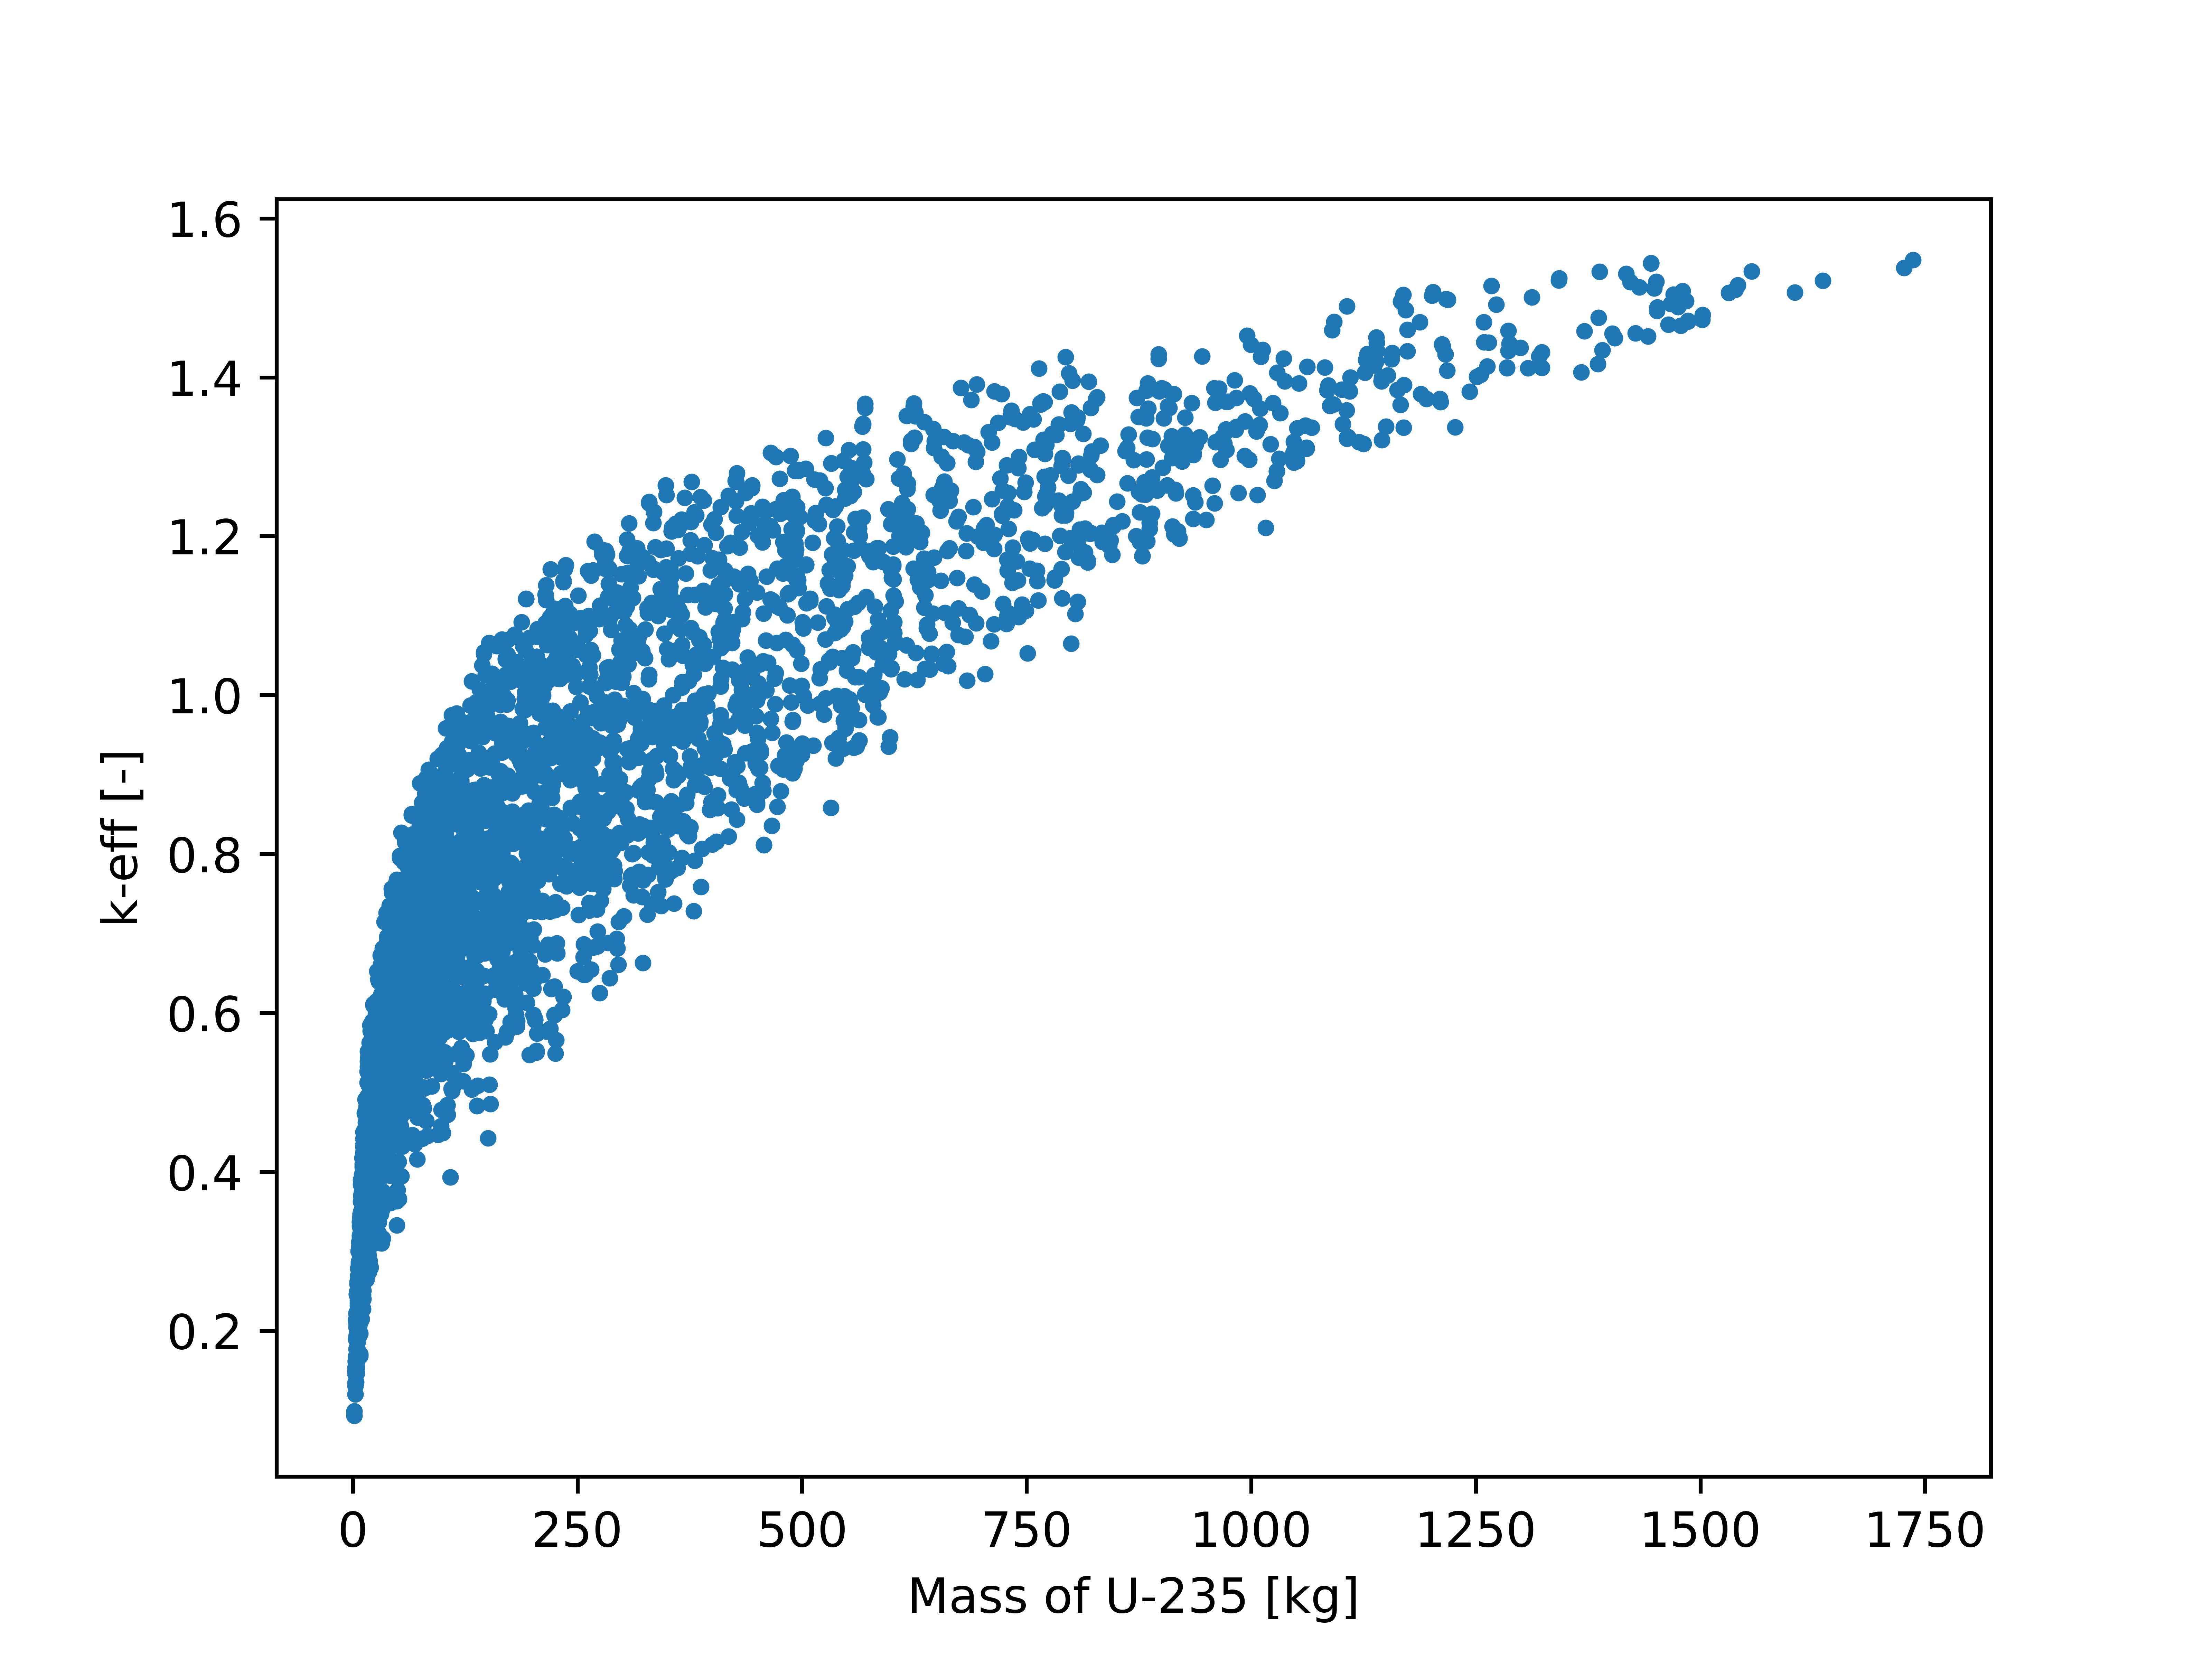
\includegraphics[width=3in]{../images/keff_vs_mass_235.png}
\caption{EOL \keff dependence on \uran mass}
\label{fig:eol_keff_vs_235_mass}
\end{figure}

This conclusion was useful for modeling a reactor's mass. Since EOL \keff is
dependent on \uran mass, for a fixed enrichment, EOL \keff can be modeled by
using the few parameters that affect reactor mass.

\subsection{Core Radius}
Core radius has a strong impact on EOL \keff. Fuel mass was directly correlated
to fuel fraction and core volume. For a fixed aspect ratio of 1, core volume was
a cubic function of core radius. This made EOL \keff strongly dependent on core
radius. Figure \ref{fig:eol_keff_vs_r_core} shows the correlation between 
core radius and EOL \keff. There was a strong relationship between core radius
and fuel mass, increasing fuel mass increased EOL \keff.

\begin{figure}[h]
    \centering
    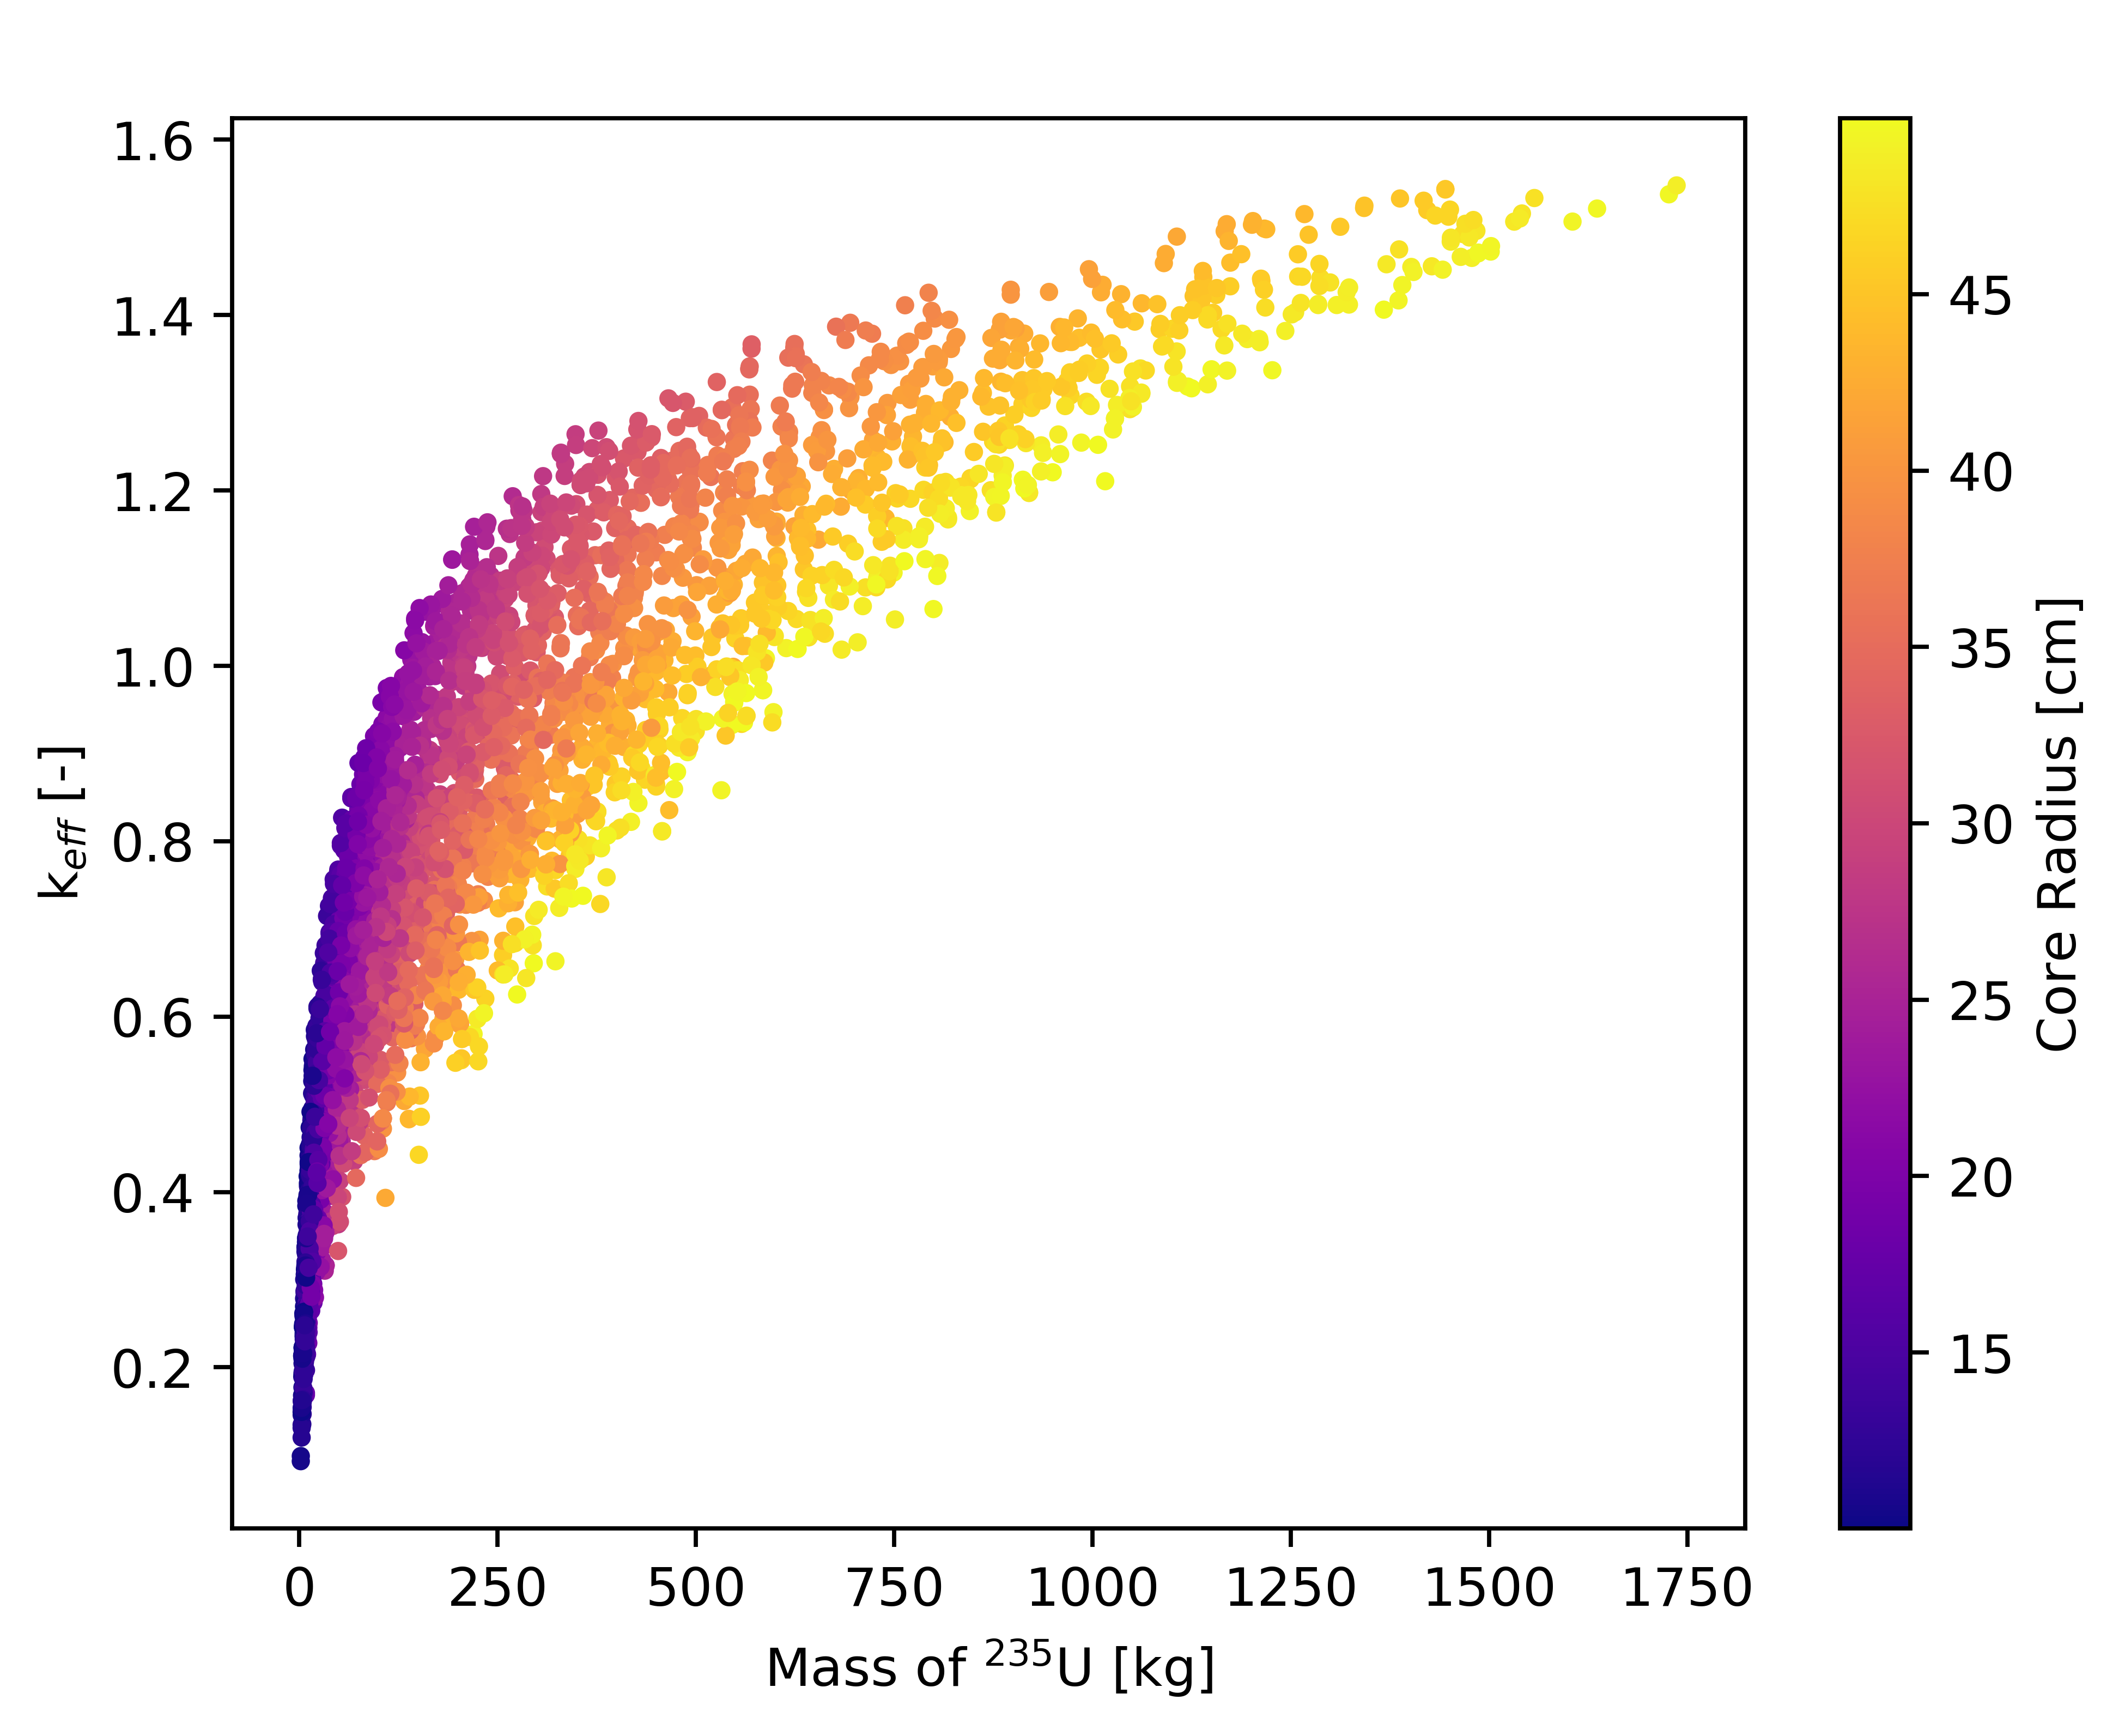
\includegraphics[width=3in]{../images/keff_vs_mass_235_core_r.png}
\caption{EOL \keff dependence on core radius.}
\label{fig:eol_keff_vs_r_core}
\end{figure}

\subsection{Fuel Enrichment}
Fuel enrichment directly affects \uran mass in nuclear fuel. Higher enrichments
yield more \uran mass for a fixed mass of fuel. Figure
\ref{eol_keff_vs_mass_enrich} shows how increasing enrichment increased \uran
mass and EOL \keff. For fixed \uran masses, increasing fuel mass also impacted
reactivity. For fixed \uran masses, higher enriched cores had greater \uran
density and as a result, higher EOL \keff.

\begin{figure}[h]
    \centering
    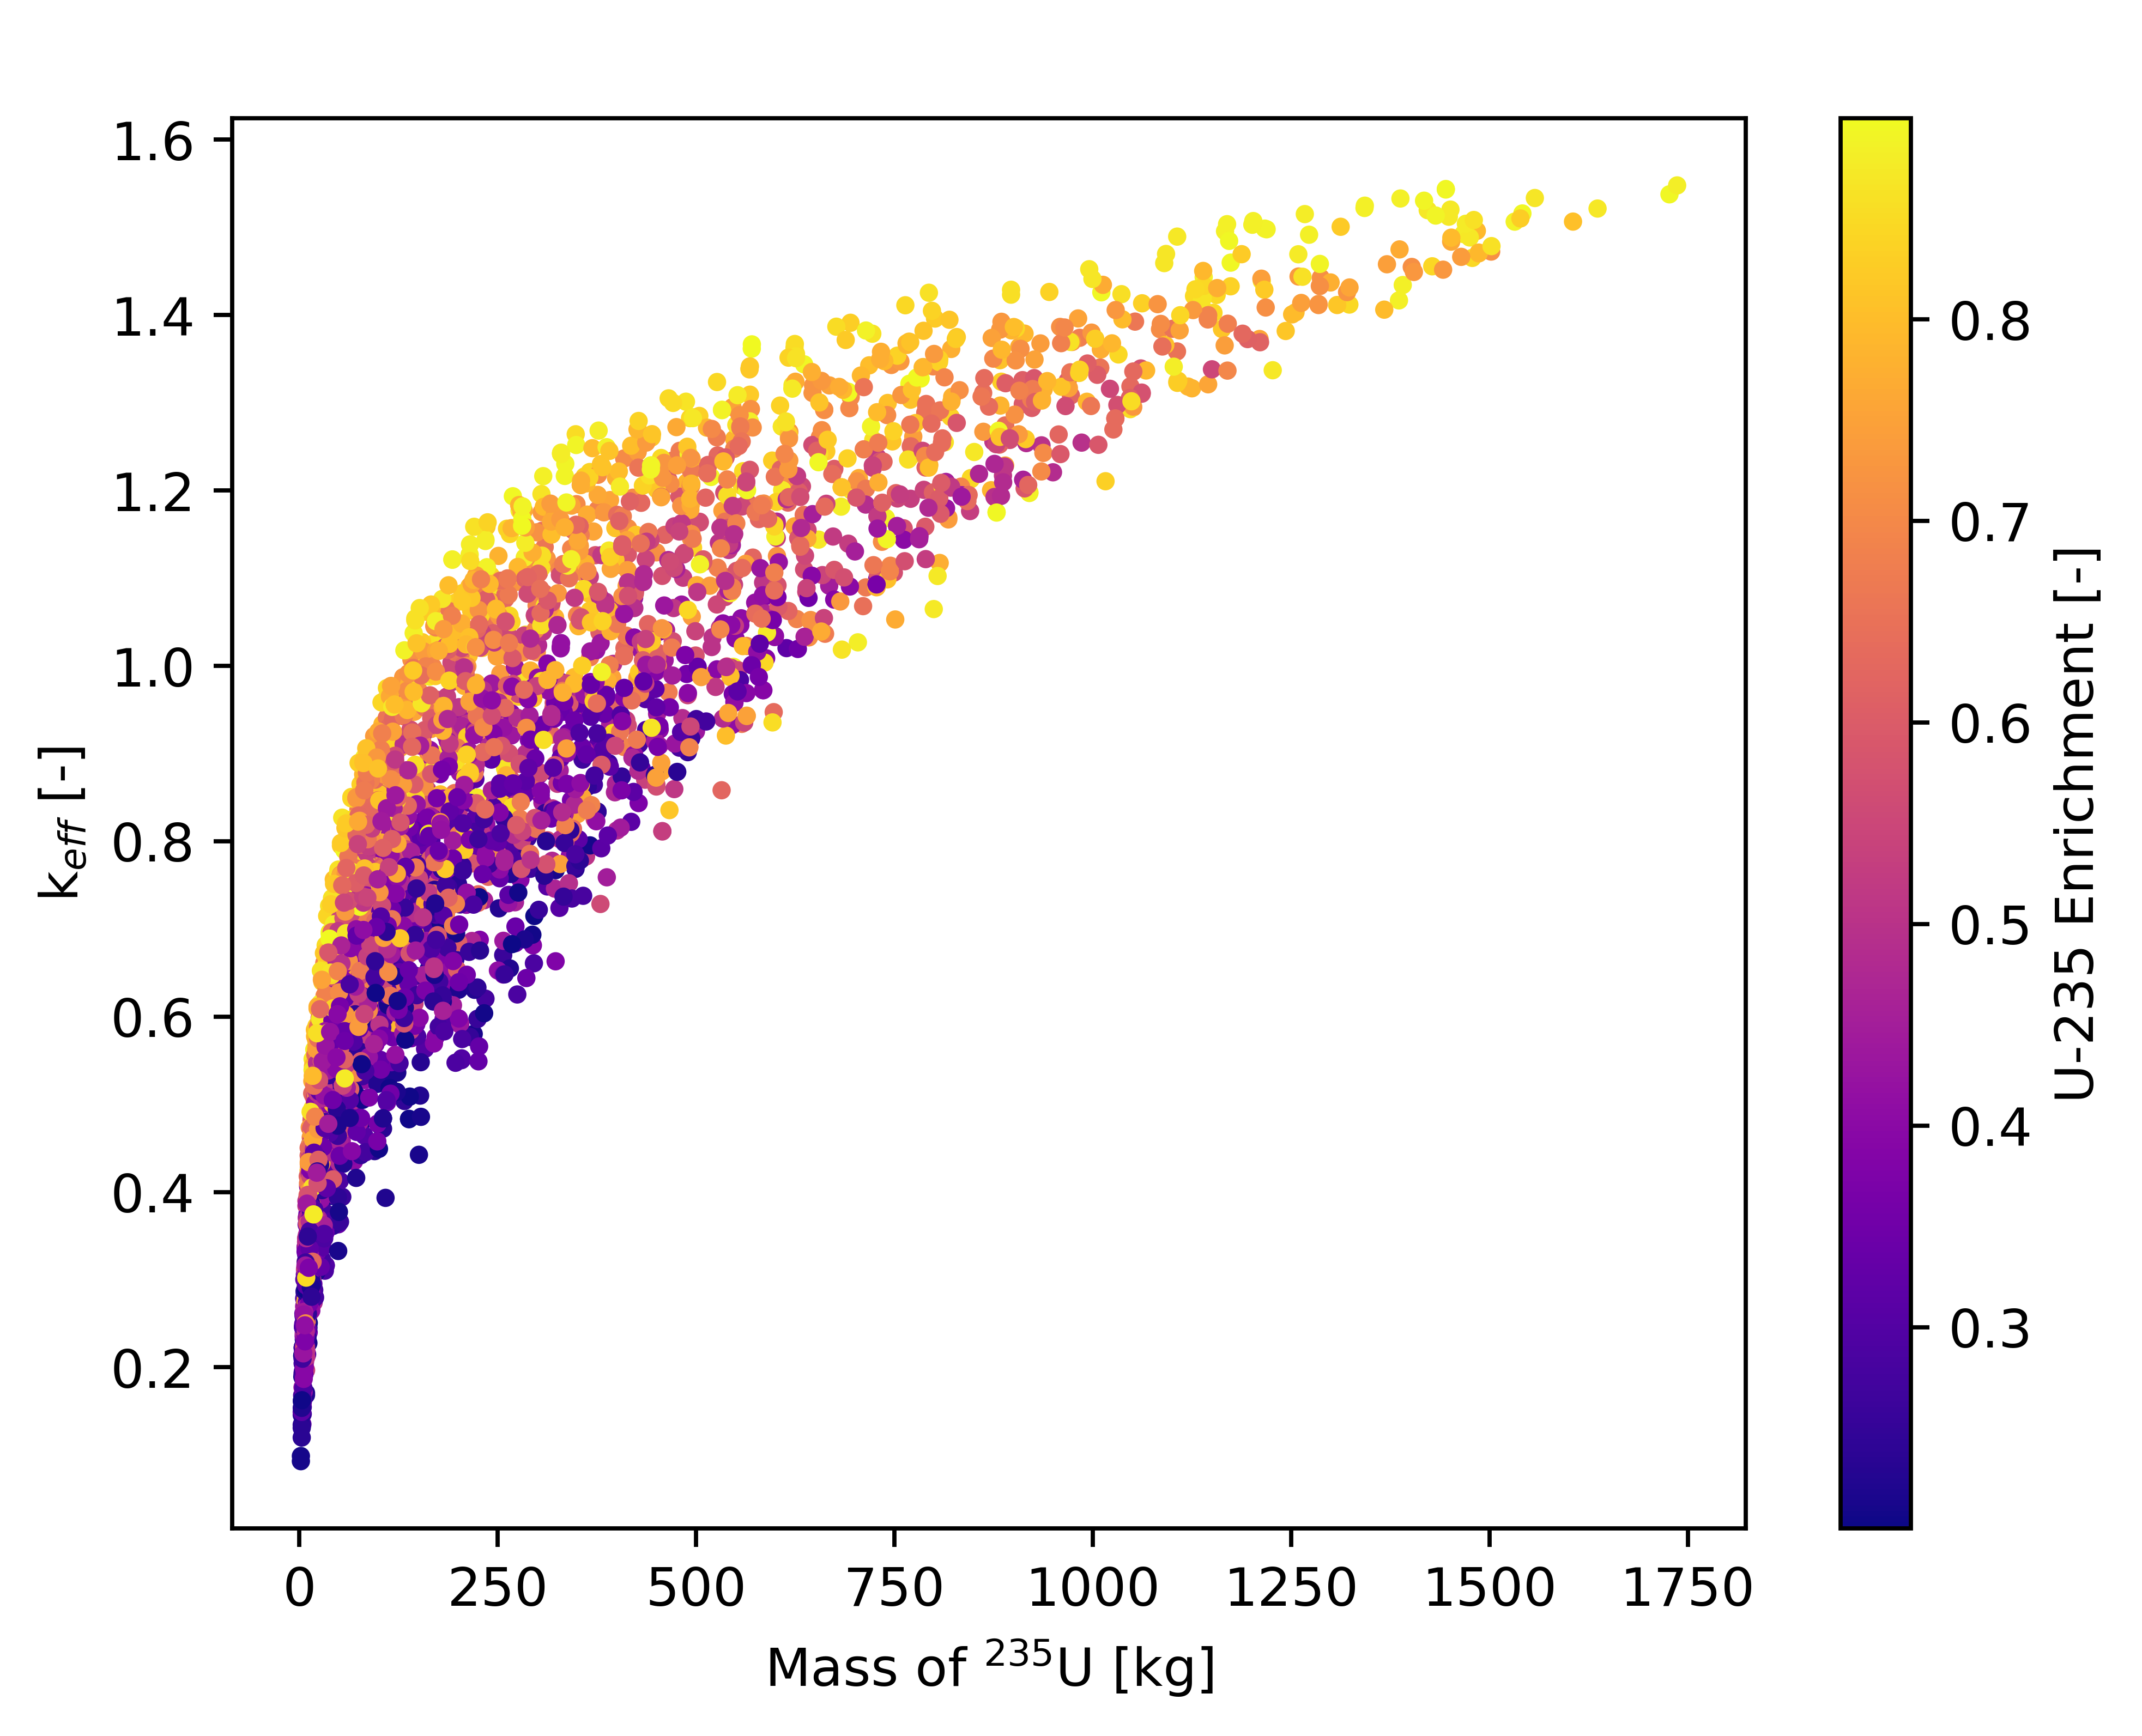
\includegraphics[width=3in]{../images/keff_vs_mass_235_enrich.png}
\caption{EOL \keff dependence on fuel enrichment}
\label{fig:eol_keff_vs_mass_enrich}
\end{figure}

\subsection{Fuel Pitch to Coolant Channel Diameter}
The fuel pitch to coolant channel diameter ratio (PD) also directly impacts
\uran mass in fuel. PD affects volumetric fuel fraction. Figure
\ref{fig:eol_keff_vs_PD_mass} shows the impact of PD on \uran mass and EOL
\keff. In addition to increasing \uran mass, PD impacts uranium density.
Reactors with larger PD ratios had greater \uran density which reduced neutron
leakage from the core and increased EOL \keff.

\begin{figure}[h]
    \centering
    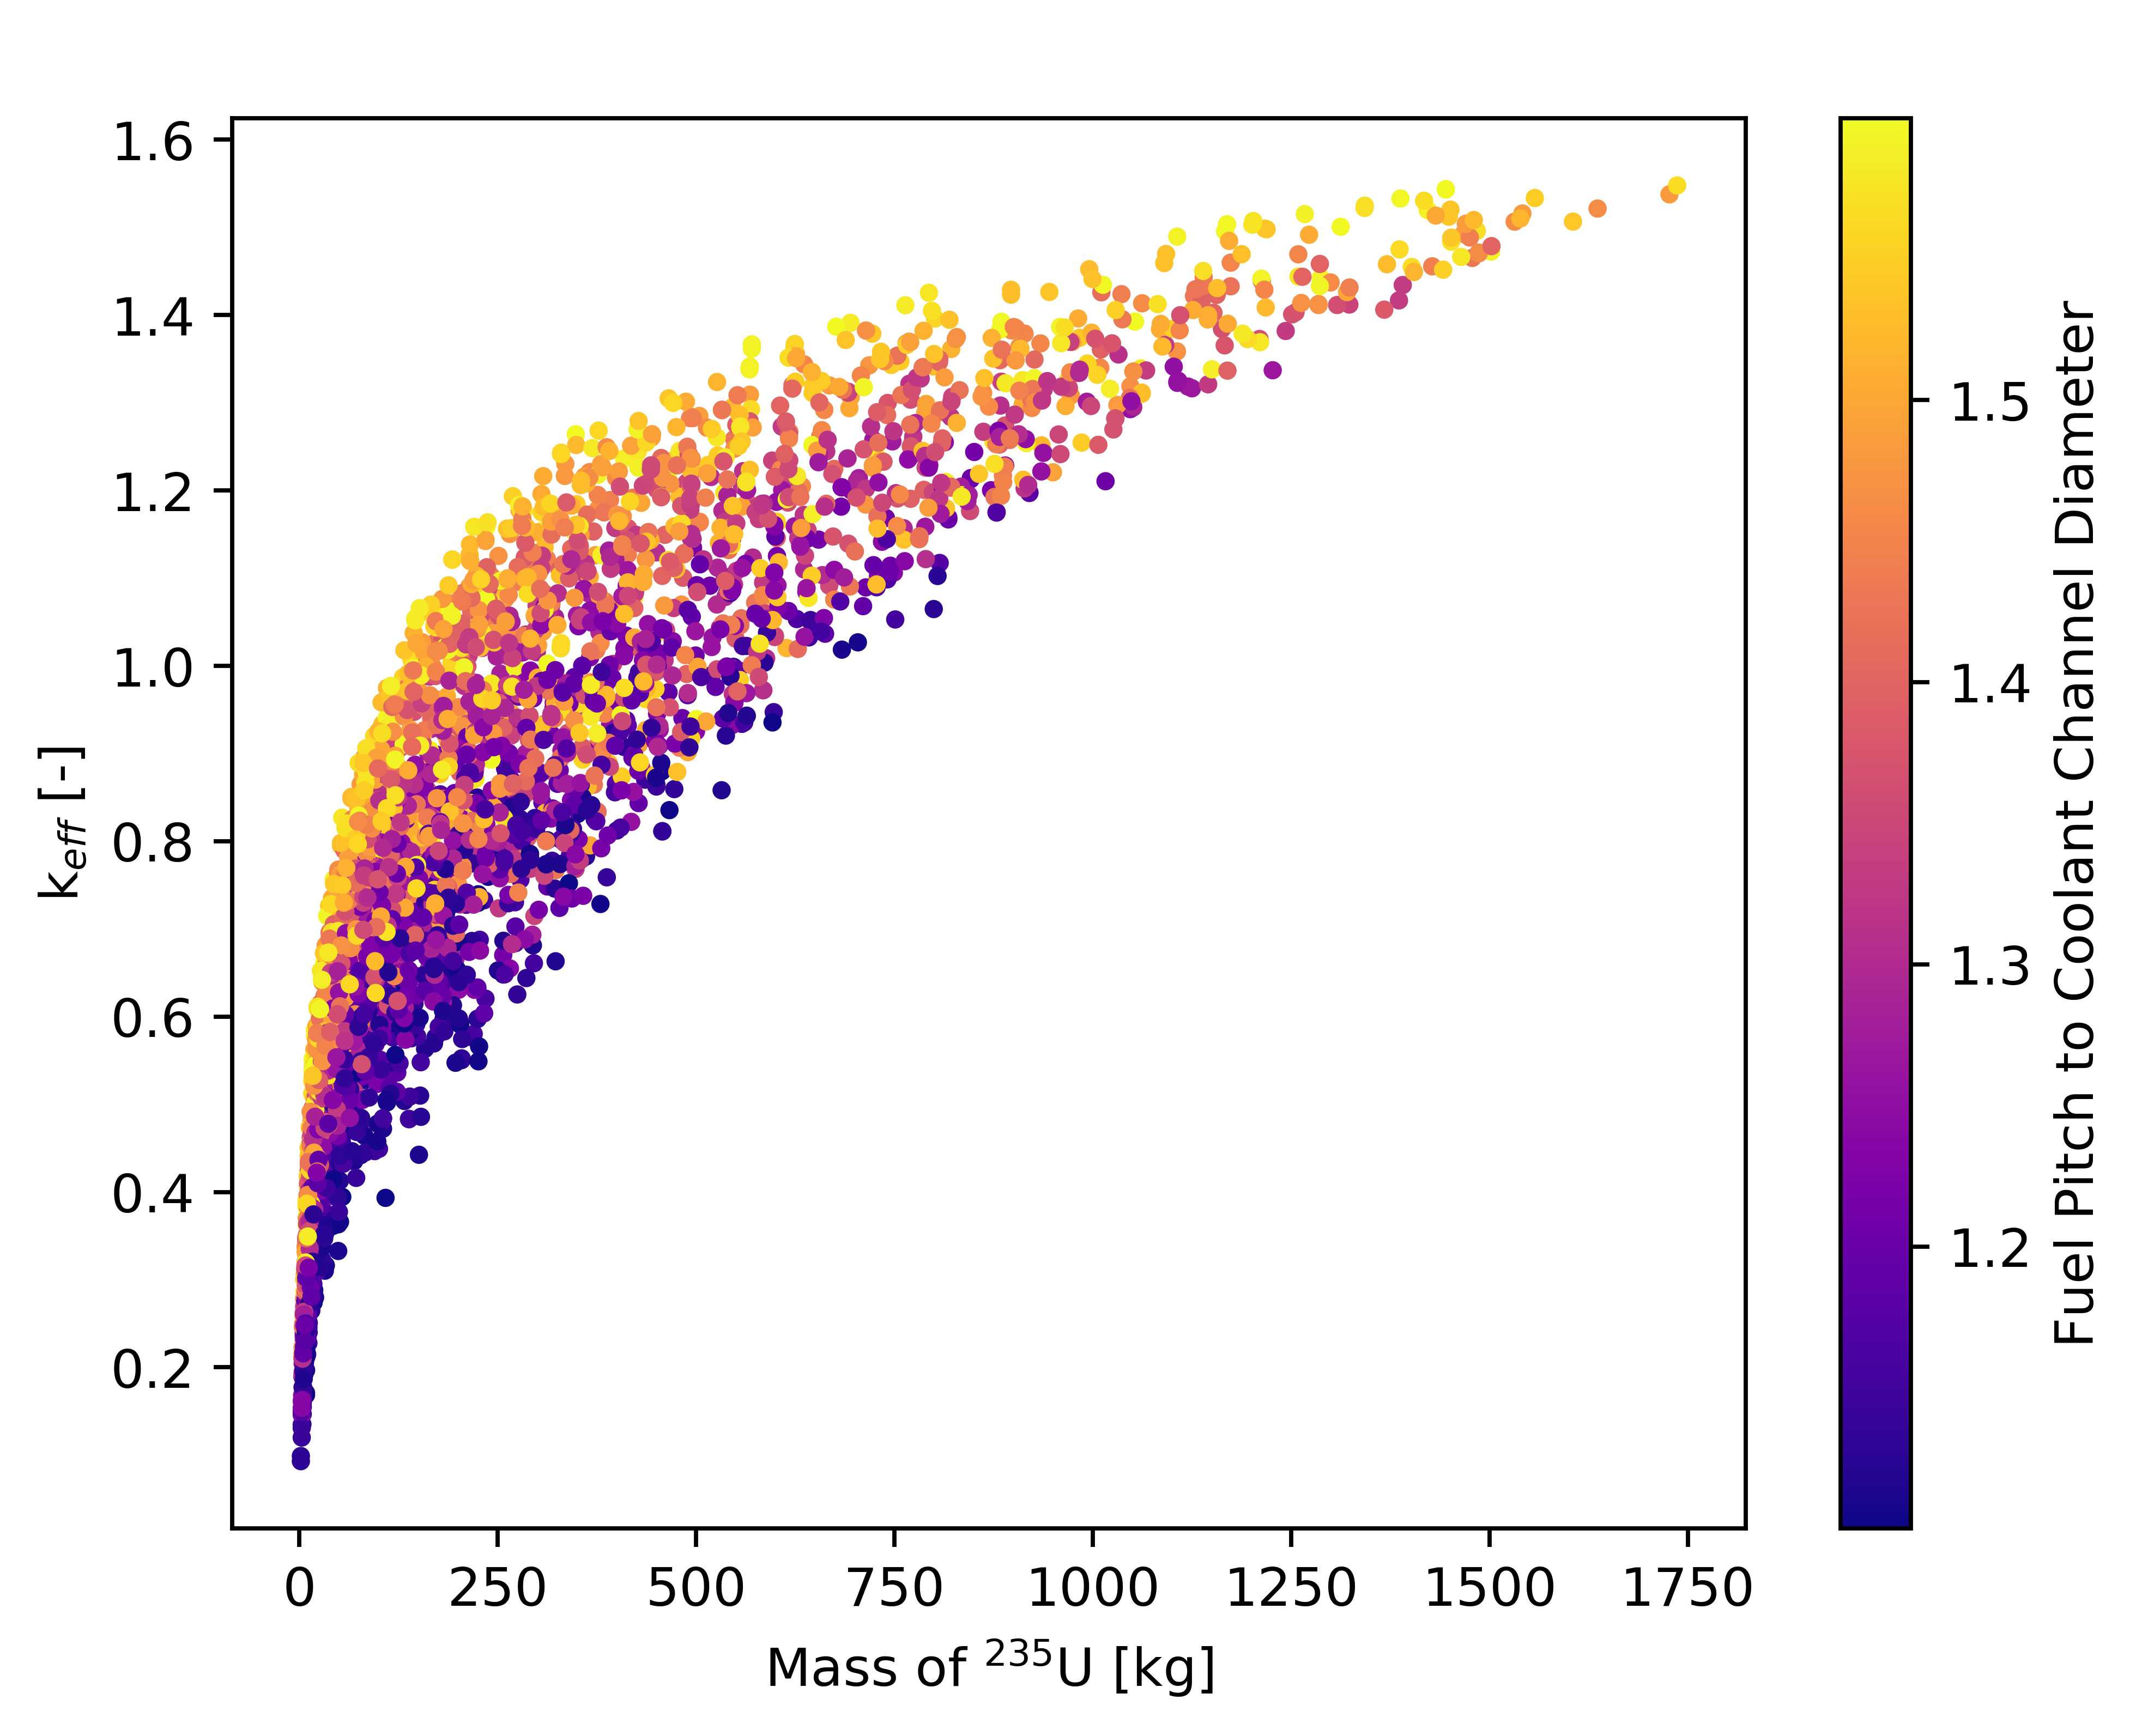
\includegraphics[width=3in]{../images/keff_vs_mass_235_PD.png}
\caption{EOL \keff dependence on fuel pitch to coolant channel ratio}
\label{fig:eol_keff_vs_PD_mass}
\end{figure}

\subsection{Coolant Channel Radius}
EOL \keff is independent of coolant channel radius. Channel radius had no impact
on fuel mass and small geometric features had little importance for high 
energy neutrons. Figure \ref{fig:eol_keff_vs_r_cool} shows the impact of 
coolant channel radius on EOL \keff.

\begin{figure}[h]
    \centering
    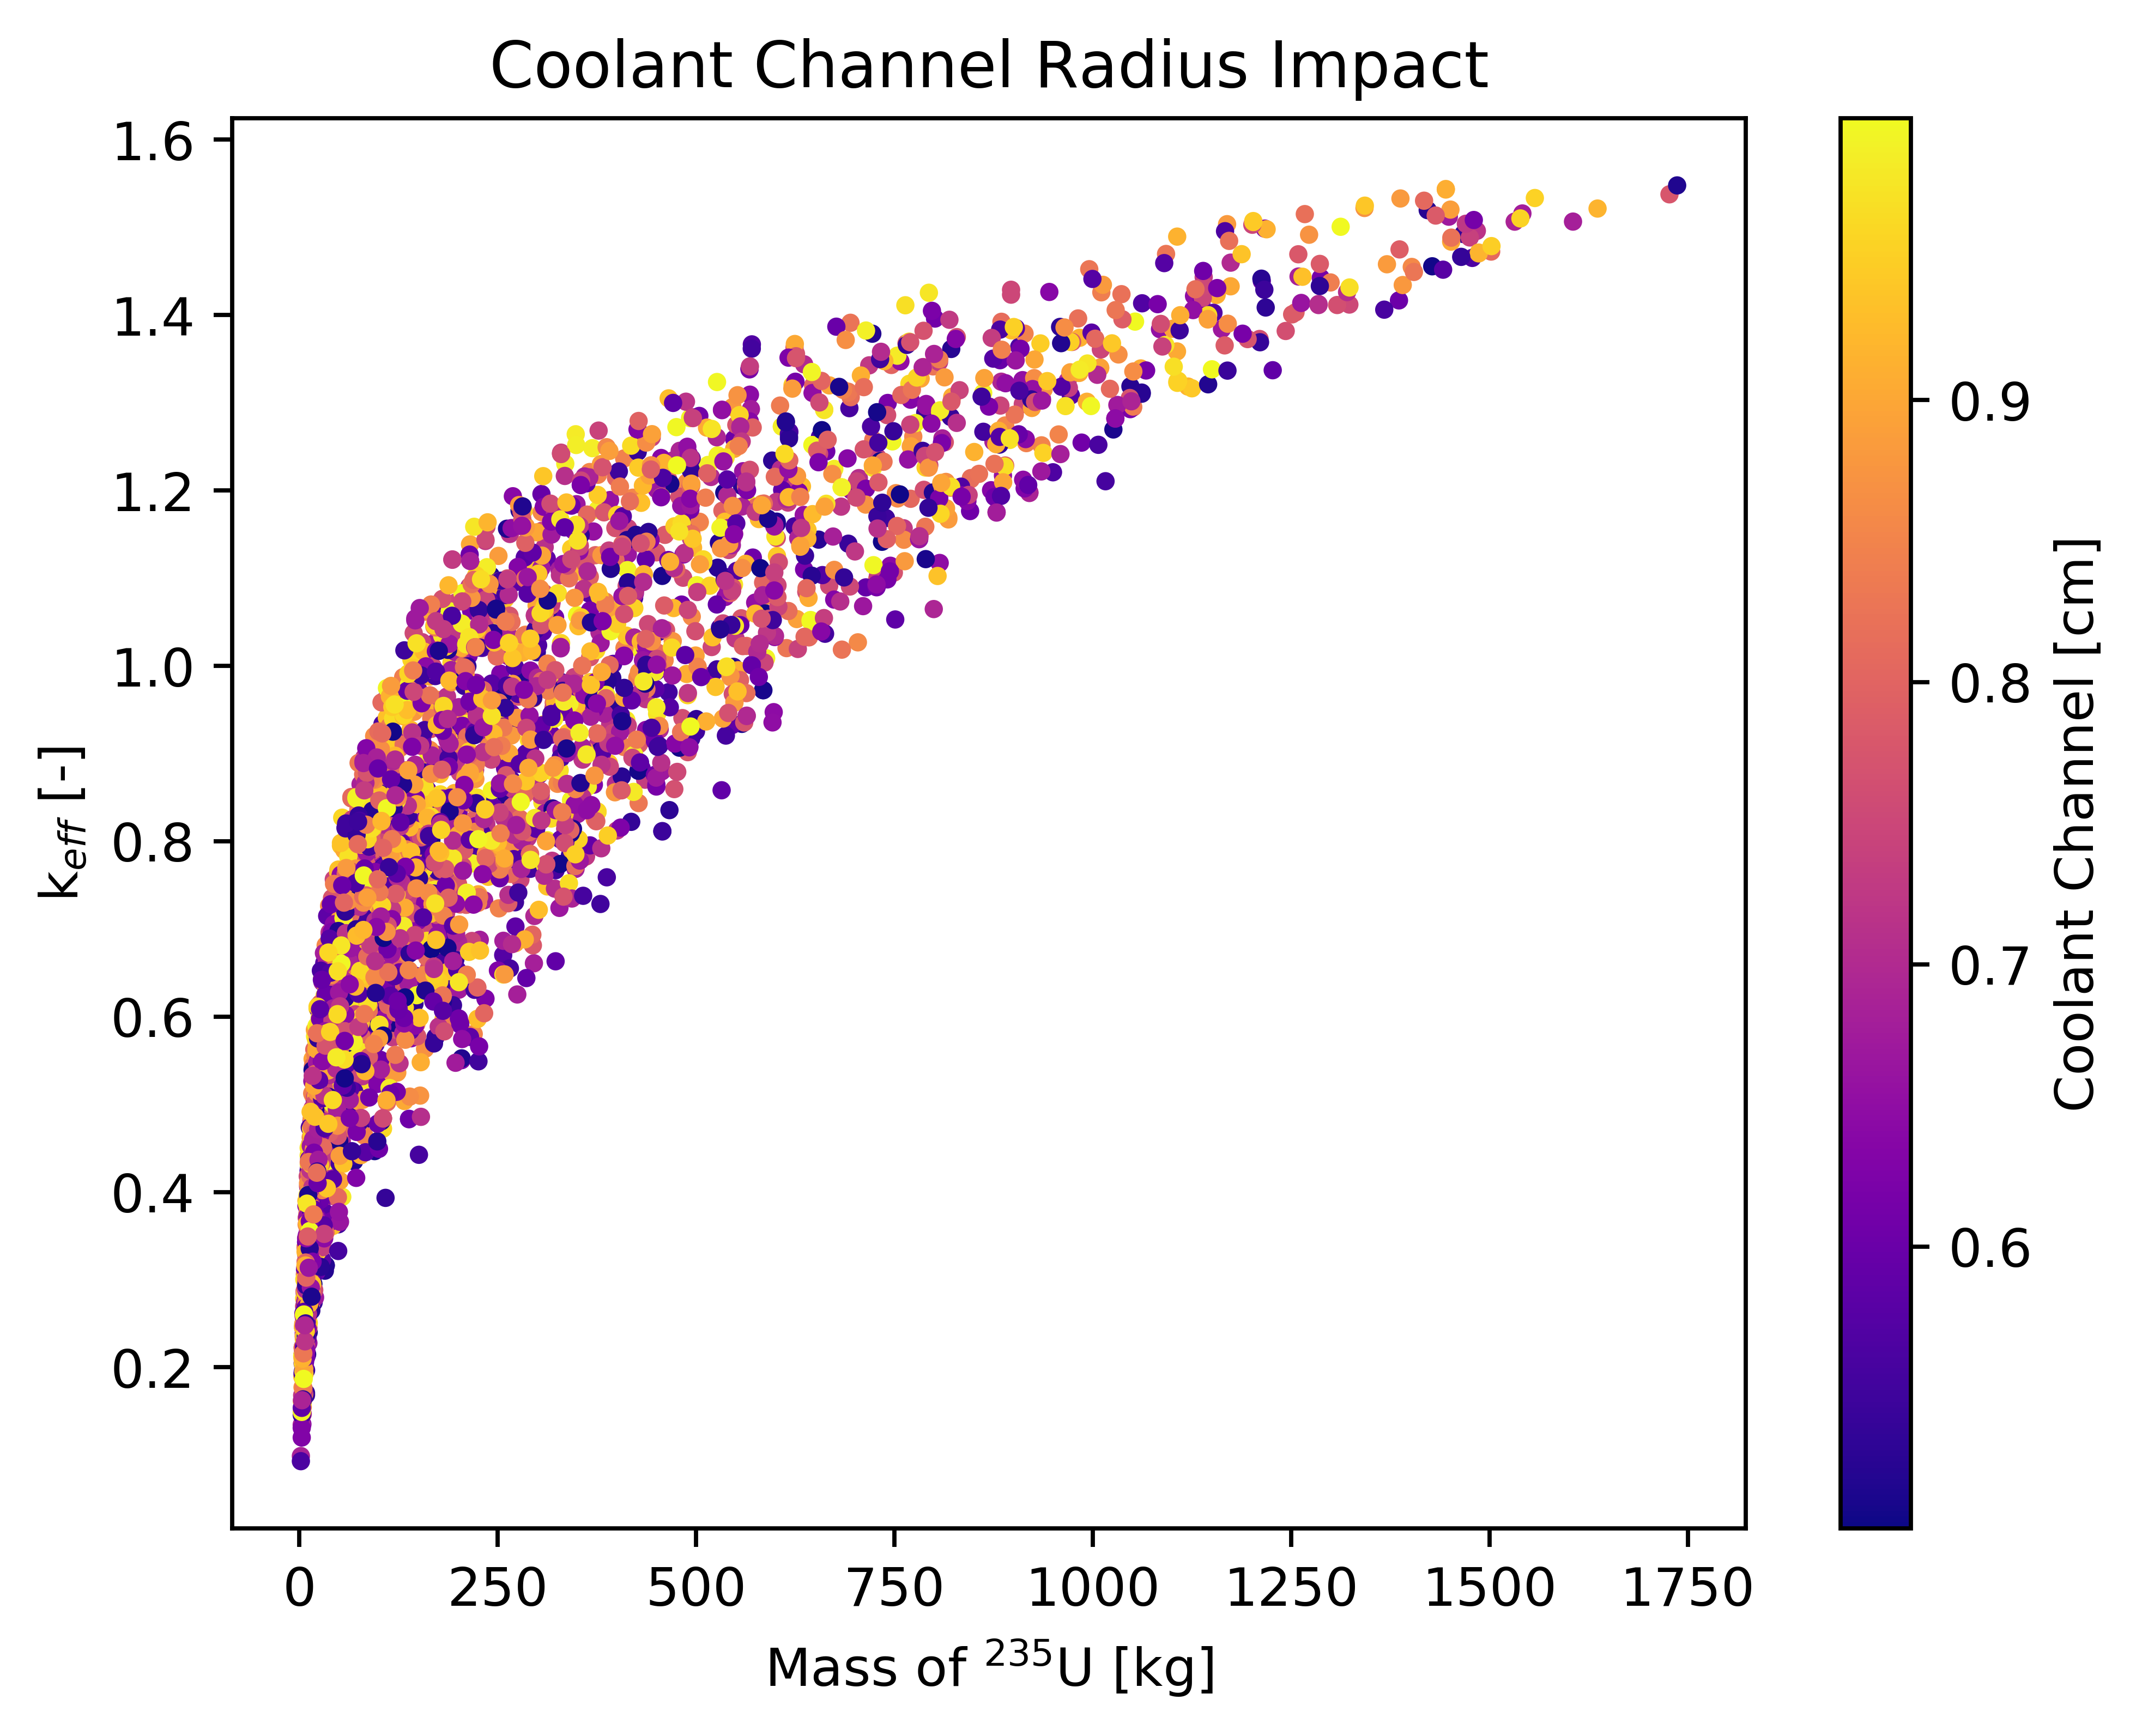
\includegraphics[width=3in]{../images/keff_vs_cool_r.png}
\caption{EOL \keff dependence on coolant channel radius}
\label{fig:eol_keff_vs_r_cool}
\end{figure}

\subsection{Thermal Power}
EOL \keff is relatively independent of thermal power.
Figure \ref{fig:eol_keff_vs_power} shows the relationship between thermal power
and EOL \keff.

\begin{figure}[h]
    \centering
    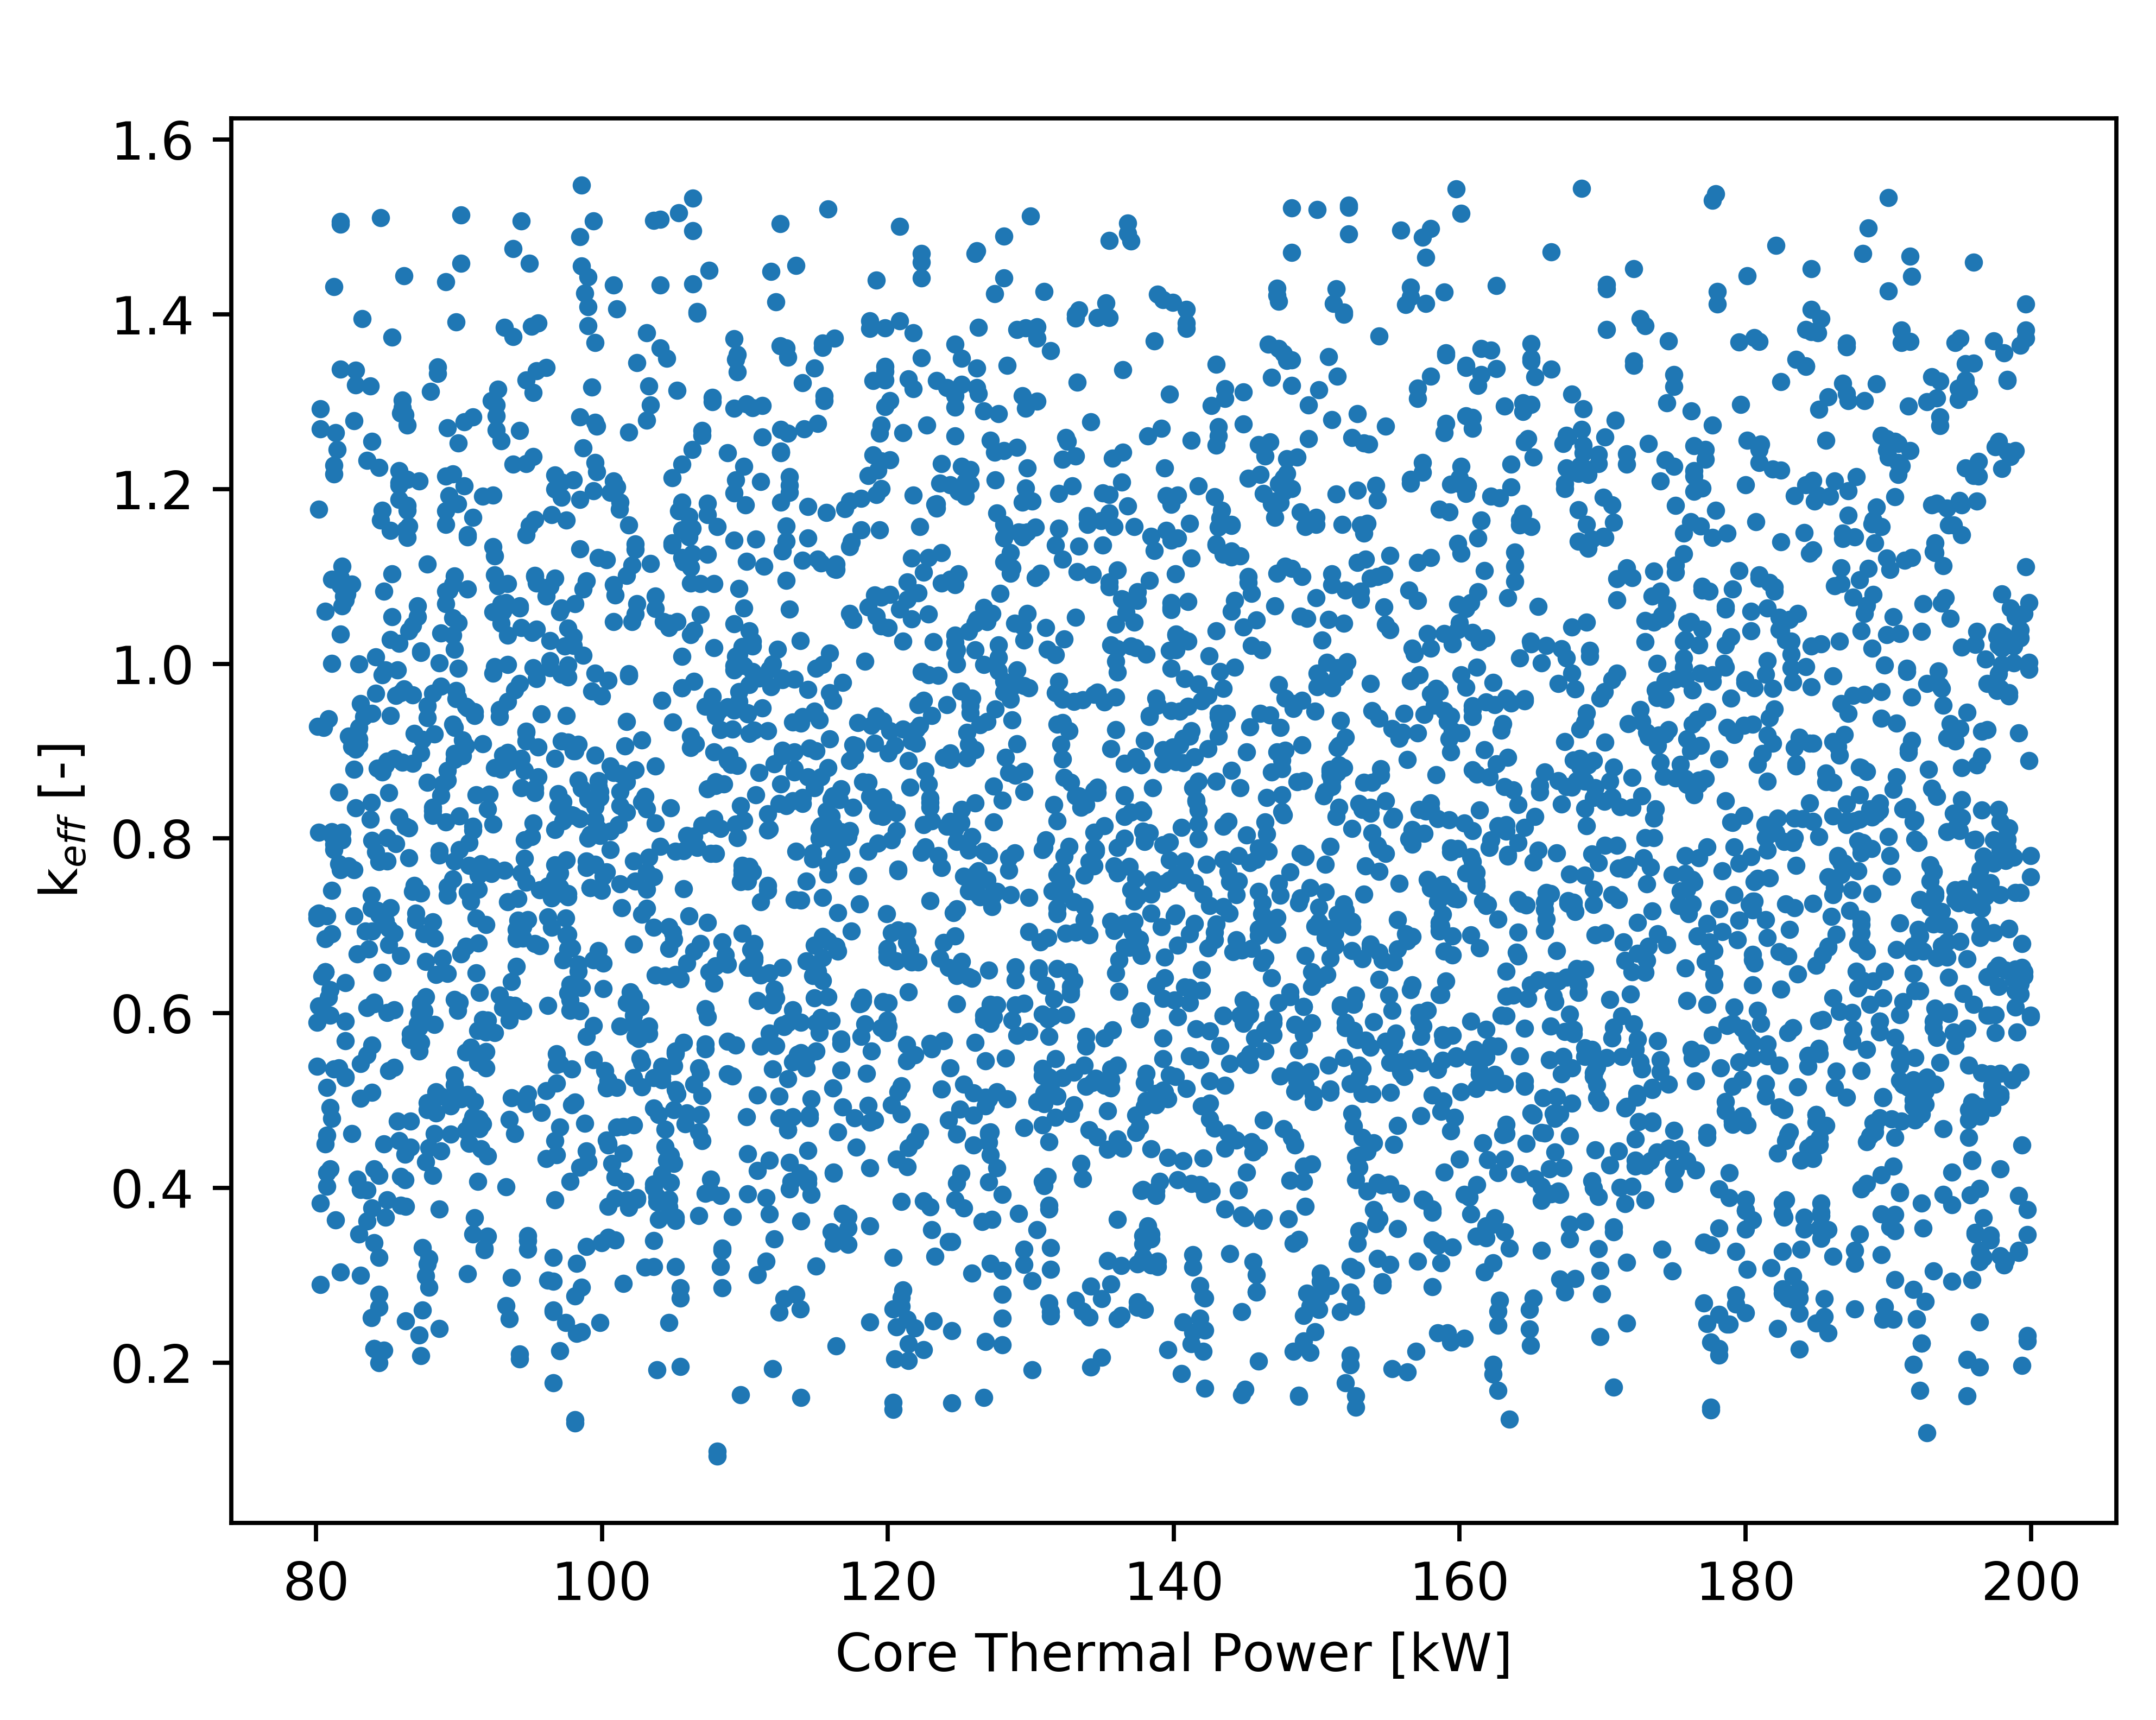
\includegraphics[width=3in]{../images/keff_vs_power.png}
\caption{EOL \keff dependence on thermal power}
\label{fig:eol_keff_vs_power}
\end{figure}

As shown in Figure \ref{fig:eol_keff_vs_power}, EOL \keff was independent of core
thermal power. The depletion mass of uranium was negligigle compared to the mass 
of uranium required for the reactor to be critical at BOL. This was confirmed
with a quick calculation. Assuming a thermal power of 150 kW for 10 years and
192 MeV per fission, the depleted mass (dU) of \uran could be calculated.

\begin{equation}
    dU = \frac{1.5x10^5\:J}{s}\;\frac{3.156x10^8\:s}{1}\;\frac{1\:
    fiss}{3.076x10^{-11}\:J}\;\frac{1\:mol}{6.022x10^{23}\:fiss}\;\frac{235\:
    g}{mol}
\end{equation}

At 150 kW of fission power, the reactor depletes approximately 600 grams of
\uran. This is a negligible mass compared to the BOL mass of a typical reactor
core (~100-500 kg). Thermal power was not a strong predictor of EOL criticality.

\section{Parametric Study Conclusion}
The purpose of this parametric study was to perform a rudimentry feature
selection. Feature selection is a technique used in machine learning and
statistics to select relevant variables (features) in a data set to simplify the
modeling of the data set. The parametric study helped identify key predictors
for the neutronic performance of a reactor design.

The figure of merit for neutronics performance was EOL \keff. The reactor must
sustain a fission chain reaction throughout the mission lifetime. In order to
ensure the reactor mass model generates a neutronically viable core, it was
necessary to determine on which input parameters EOL \keff is most strongly
dependent. To support this analysis, 3901 MCNP6.1 depletion calculations were
performed over a 5-dimensional sample space with Latin Hypercube Sampling
techniques to ensure even sampling. The conclusion of this work is that fissile
material mass is the most important parameter to predict EOL \keff. Another
important conclusion was that EOL \keff is relatively independent of thermal power. This
meant EOL \keff could be estimated as BOL \keff adjusted for marginal burnup.
This conclusion was useful to constrain reactor parameters and will be utilized
in Chapter \ref{ch:crit_radius} to justify a relationship between core fuel fraction
and a required core radius to ensure EOL \keff > 1.0.
